\renewcommand{\thechapter}{6}

\chapter{Ionization and Scintillation Yield}
\label{Ch:LYQY}

The goal of the following two sections is to extract light yield, charge yield and recombination fluctuations from the tritium spectrum using the methods described in section \ref{sec:flucs_mono_bins}. The first step is to use the NEST model in an attempt to undue the effect of the tritium spectral shape and finite detector resolution, described in this section. We find that the light yield and charge yields extracted from the data deviate too much to apply the correction factor. Since the correction is found to be small we can proceed to extract new LY, QY and $\rm \sigma R$ from the tritium data without correction building a model that better reproduces the data than the NEST model (which has yet to be vetted at our electric field and energy). We then take that improved model and apply the correction.



\section{Measuring LY, QY and Recombination, Uncorrected for Spectral shape}

\subsection{Tritium S1 Mean and NEST}

The correction for the mean of the measured light yield, S1 [Phe], for tritium beta decay can be solved for using equation \ref{eq:5}. Starting with a simulated S1 tritium spectrum with infinite resolution and applying equations \ref{eq:1}-\ref{eq:5} one can attain the mapping of measured mean to true mean. The resolution of S1 was determined from statistical and  instrumental fluctuations and is given in equation \ref{eq:SigStat} and \ref{eq:SigInst}. The use of Gaussian error down to low S1 is an acceptable approximation since underlying distribution actually consists of the number of photons, $\rm n_\gamma = \frac{S1}{g1}$. With g1=0.097 there are still 20 photons near the S1 threshold of 2 [Phe], thus the Gaussian model is still a close approximation of the underlying Poisson distribution. We will use the Gaussian approximation as it makes the application of equations \ref{eq:1}-\ref{eq:5} much simpler.
The variance in S1 is the result of recombination fluctuations, statistical fluctuations and instrumental fluctuations at a given energy. The functional form of all three have been previously measured and can be extrapolated for use with the tritium spectrum. The first step is to use the expected light yields from NEST along with the measured smearing from recombination and detector resolution to extract a correction factor for the observed S1 signal. Having a priori knowledge of light yields will allow for the spectral shape to be corrected or can at least be used to approximate an error when we go to extract the light yield and recombination fluctuations from the tritium beta spectrum.

\begin{equation}
 \rm \sigma_{S1}^2=g_1^2(\sigma_{n_{\gamma_{stat}}}^2+\sigma_{n_{\gamma_{inst}}}^2+\sigma_R^2)
\label{eq:S1_res}
\end{equation}

Figure \ref{fig:S1_mapping} shows the application of smearing  from equation \ref{eq:S1_res} applied to the expected S1 tritium spectrum from NEST overlaid with the data. The mapping for converting the observed S1 to the real S1 is shown in figure \ref{fig:S1_mapping}. To calculate the correction we start with the NEST light yield, apply the measured g1, convolve it with a tritium beta spectrum and add in our first approximation of recombination fluctuations measured in equation \ref{eq:Inst_Fit}, given infinite detector resolution this is the spectrum the LUX detector would observe in S1 space. Knowing the dependance of detector resolution vs. the number of photons of a given event (equation \ref{eq:SigDet}) we can apply the model as outlined in \ref{sec:Smear} and calculate the shift from observed mean photons to real mean photons.

 \begin{figure}[h!]\centering
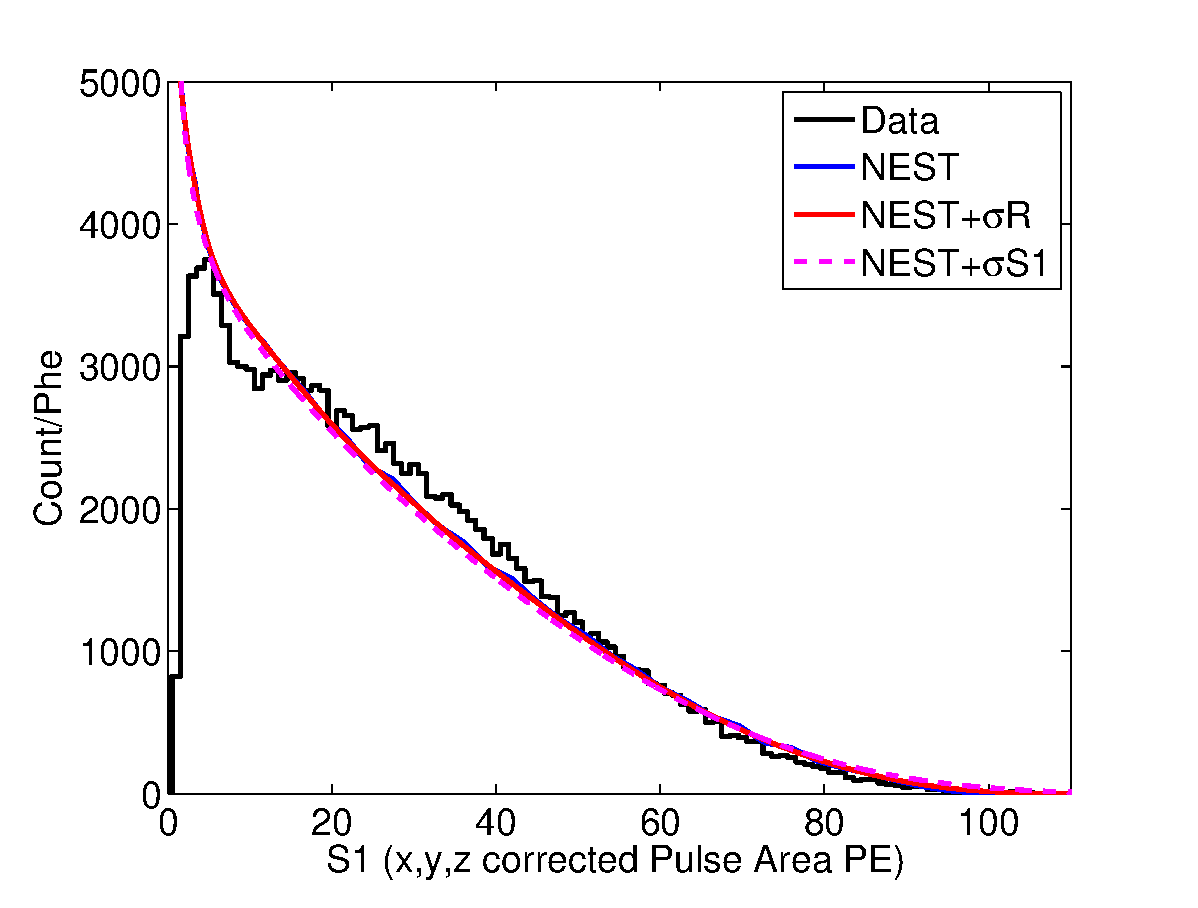
\includegraphics[width=70mm]{Chapter_Flucs/Figures/S1S2_Spectra/S1_spec_compare_.eps}
%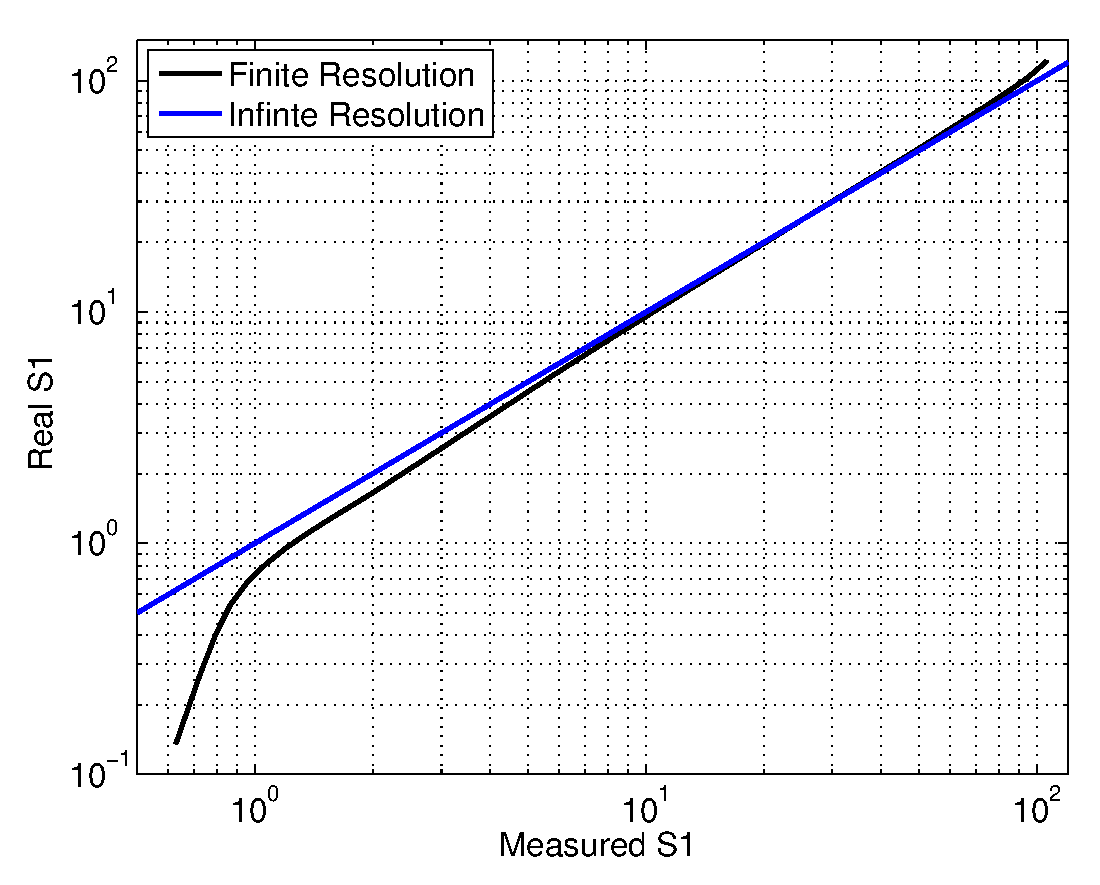
\includegraphics[width=70mm]{Chapter_Flucs/Figures/S1_smear_comp}
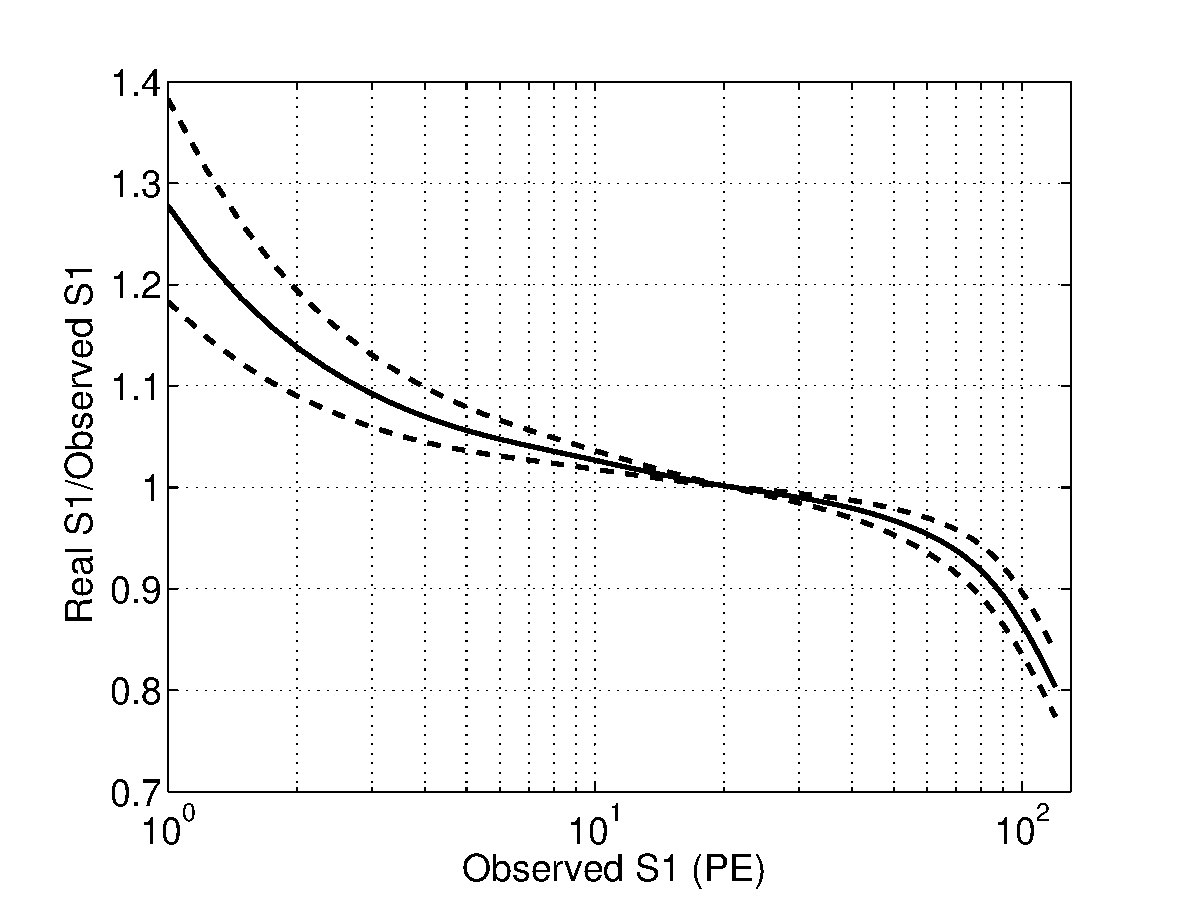
\includegraphics[width=70mm]{Chapter_Flucs/Figures/S1S2_Spectra/S1_corr_.eps}
\caption{Left: In Black S1 tritium spectrum extracted from the data. In blue, The NEST light yield curve. In red, the NEST light yield curve with recombination fluctuations. Dashed magenta is NEST light yield with smearing from equations \ref{eq:S1_res}.  Right: The ratio of the real mean to the observed mean vs. the observed mean for a tritium photon spectrum. Note the S1 threshold at about 3 Phe in S1. }
\label{fig:S1_mapping}
\end{figure}


\subsection{Tritium S2 Mean and NEST}

The correction for the mean of the measured charge yield, S2 [Phe], for tritium beta decay can be solved for using equation \ref{eq:5}. Starting with a simulated S2 tritium spectrum with infinite resolution and applying equations \ref{eq:1}-\ref{eq:5} one can attain the mapping of measured mean to true mean.  The resolution of S2 was determined from statistical and  instrumental fluctuations and is given in equation \ref{eq:SigStat} and \ref{eq:SigInst}. The use of Gaussian error down to low S2 is an acceptable approximation since the S2 spectrum ends at 300 [Phe], $\rm n_e = \frac{S2}{g2}$. With g2=5.75 there are still 50 electrons near end of the tritium spectrum, thus the Gaussian model is still a close approximation of the underlying Poisson distribution. We will use the Gaussian approximation as it makes the application of equations \ref{eq:1}-\ref{eq:5} much simpler.
As in the case of the light yield, the variance in S2 is the result of recombination fluctuations, statistical fluctuations and instrumental fluctuations at a given energy. The functional form of all three have been previously measured and can be extrapolated for use with the tritium spectrum. We first use the expected charge yields from NEST along with the measured smearing from recombination and detector resolution to extract a correction factor for the observed S2 signal. Having a priori knowledge of light yields will allow for the spectral shape to be corrected or can at least be used to approximate an error when we go to extract the charge yield and recombination fluctuations  from the tritium beta spectrum.

\begin{equation}
 \rm \sigma_{S2}^2=g_2^2(\sigma_{n_{e_{stat}}}^2+\sigma_{n_{e_{inst}}}^2+\sigma_R^2)
\label{eq:S2_res}
\end{equation}


Figure \ref{fig:S2_mapping} shows the application of smearing from equation \ref{eq:S2_res} applied to the S2 tritium spectrum expected from NEST overlaid with the data. As with the S1 spectrum the correction is calculated using NEST for charge yield with the measured g2 applied, convolve it with a tritium beta spectrum and using our first approximation of recombination fluctuations measured in equation \ref{eq:Inst_Fit}, given infinite detector resolution this is the spectrum the LUX detector would observe in S2 space. Having calculated the dependance of detector resolution vs. the number of photons of a given event (equation \ref{eq:SigDet}) we can apply the smearing as outlined in \ref{sec:Smear} and calculate the shift from observed mean photons to real mean photons. From the S2 spectrum, which is more peaked than the S1, we see the ~20\% discrepancy with the NEST charge yield model but it may also be an indication of the error in g1 and g2.

 \begin{figure}[h!]\centering
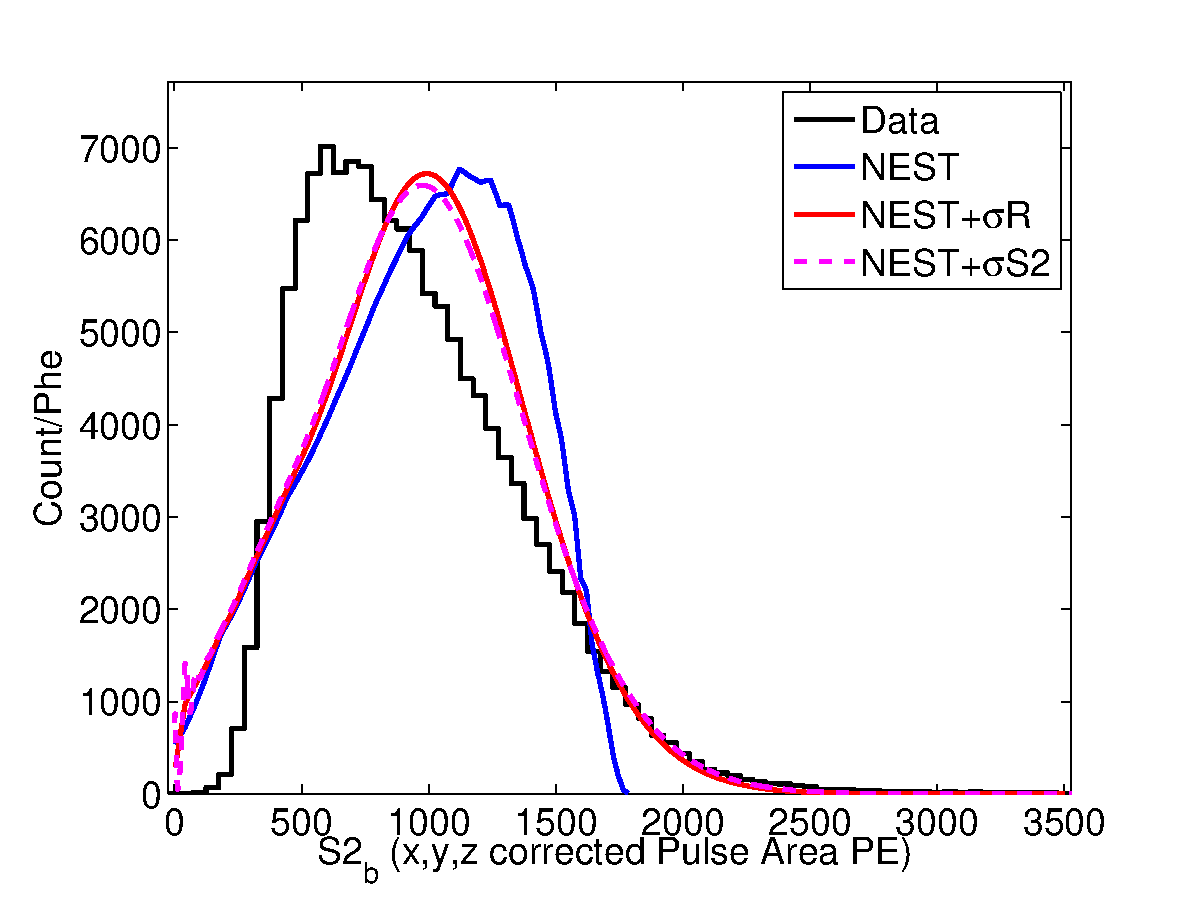
\includegraphics[width=70mm]{Chapter_Flucs/Figures/S1S2_Spectra/S2_spec_.eps}
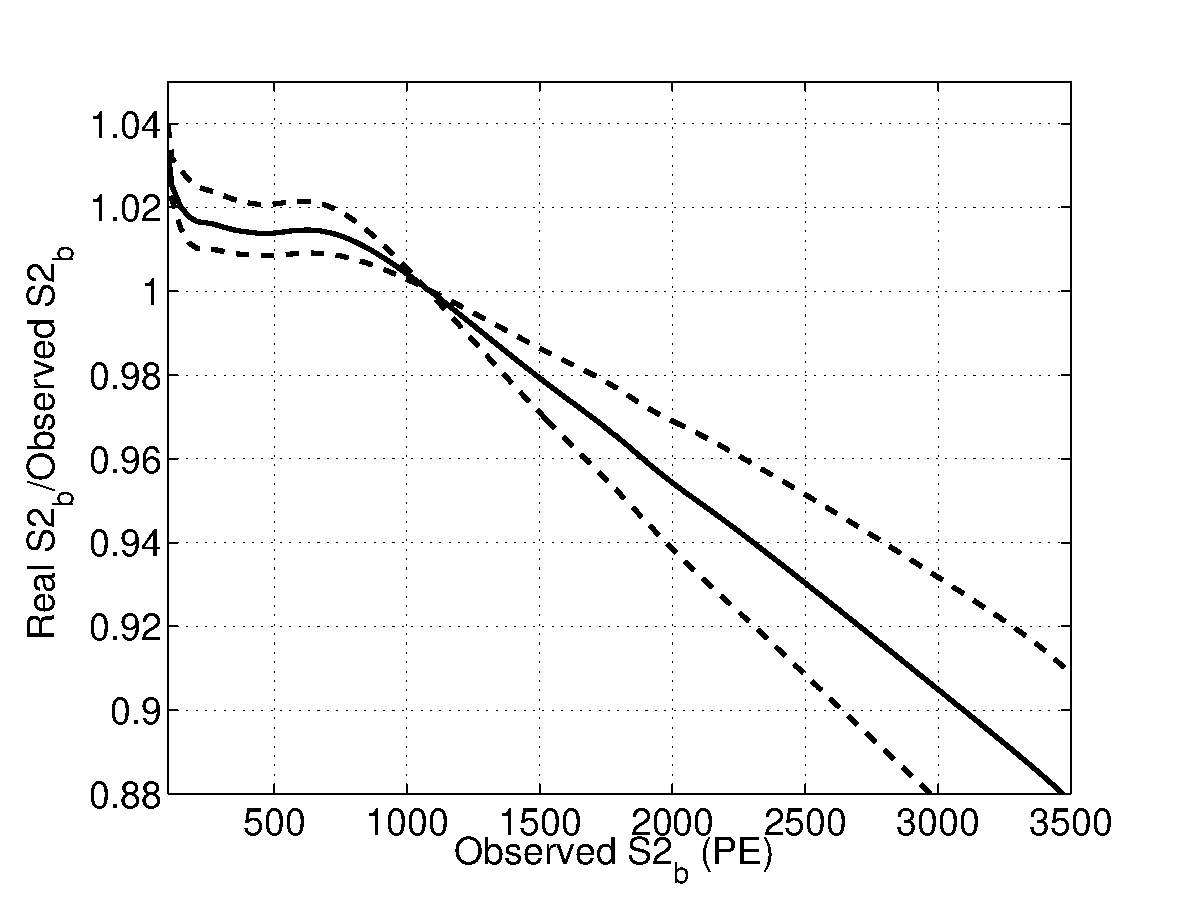
\includegraphics[width=70mm]{Chapter_Flucs/Figures/S1S2_Spectra/S2_corr_.eps}
\caption{Left: In Black S2 tritium spectrum extracted from the data. In blue, The NEST light yield curve. In red, the NEST light yield curve with recombination fluctuations. Dashed magenta is NEST light yield with smearing from equations \ref{eq:S2_res}.  Right: The ratio of the real mean to the observed mean vs. the observed mean for a tritium photon spectrum. Note the S2 threshold at about 400 Phe in S2. }
\label{fig:S2_mapping}
\end{figure}


\subsection{Tritium Energy Spectrum}

The mapping of the observed energy to real energy was determined using a full simulation of tritium beta decay. The accuracy of the smearing model described in equations \ref{eq:1}-\ref{eq:5} can be tested by comparing it against the energy observed after a full NEST simulation. The energy depends on both S1 and S2 thus, mapping observed energy to true energy my be non trivial. Again, we start with a simulated tritium energy spectrum with infinite resolution and apply the empirically determined resolution in equation \ref{eq:E_res}, measured with $\rm^{127}Xe$ X-rays and $\rm ^{83m}Kr$ calibrations. Figure \ref{fig:E_spec} shows the comparison of smearing model vs true energy along with the smearing after running full photon and electron propagation in LUXSIM vs the true energy. The smearing form the model described in equations \ref{eq:1}-\ref{eq:5} is almost identical to the output of LUXSIM. The energy spectrum flares out at low energy, is pulled in from 5-10 [keV] and again flares out slightly above 15 [keV]. It is important to note that the change in the spectral shape is hardly noticeable, as was the case with S1 and somewhat with S2. Figure \ref{fig:E_mapping} shows the results for mapping observed energy to real energy using both smearing methods. The two methods show good agreement down to the threshold of 1.5 [keV], the agreement with simulation is always within 1\%. Below 2 [keV] the model predicts the ratio of true energy to observed energy to rise as there are greater number of events at higher energy spilling over to lower energy, the simulation however does not show this behavior leading to a 5\% discrepancy in the 1 [keV] bin. We take the difference between the smearing model and LUXSIM as a systematic uncertainty. 

Using equation \ref{eq:Fano}, \ref{eq:Gain} and \ref{eq:E_res1} we solve for the the spread in E as a function energy \ref{eq:E_res}. $\rm a_\gamma$ and $\rm a_e$ are the coefficients in front of the root n term on the $\rm n_\gamma$ and $\rm n_e$ statistical variance . W=73 [$\rm \frac{N_{quanta}}{keV}$].

\begin{gather}
\label{eq:E_res1} \rm E= \frac{1}{W}(n_\gamma + n_{e^-}) \\
 \rm \sigma E^2= \frac{1}{W^2}(\sigma n_\gamma ^2 + \sigma n_{e^-} ^2)\\ 
 \rm \sigma E^2= \frac{1}{W^2}(a_\gamma^2 n_\gamma + a_e^2 n_{e^-})\\
 \rm \sigma E^2= \frac{(a_\gamma+a_e)^2}{W}\frac{(n_\gamma + n_{e^-})}{W}\\
 \rm \sigma E^2= \frac{(a_\gamma+a_e)^2}{W}E\\
  \rm \sigma E= \frac{(a_\gamma+a_e)}{\sqrt{W}}\sqrt{E}
\label{eq:E_res}
\end{gather}

\newpage

 \begin{figure}[h!]\centering
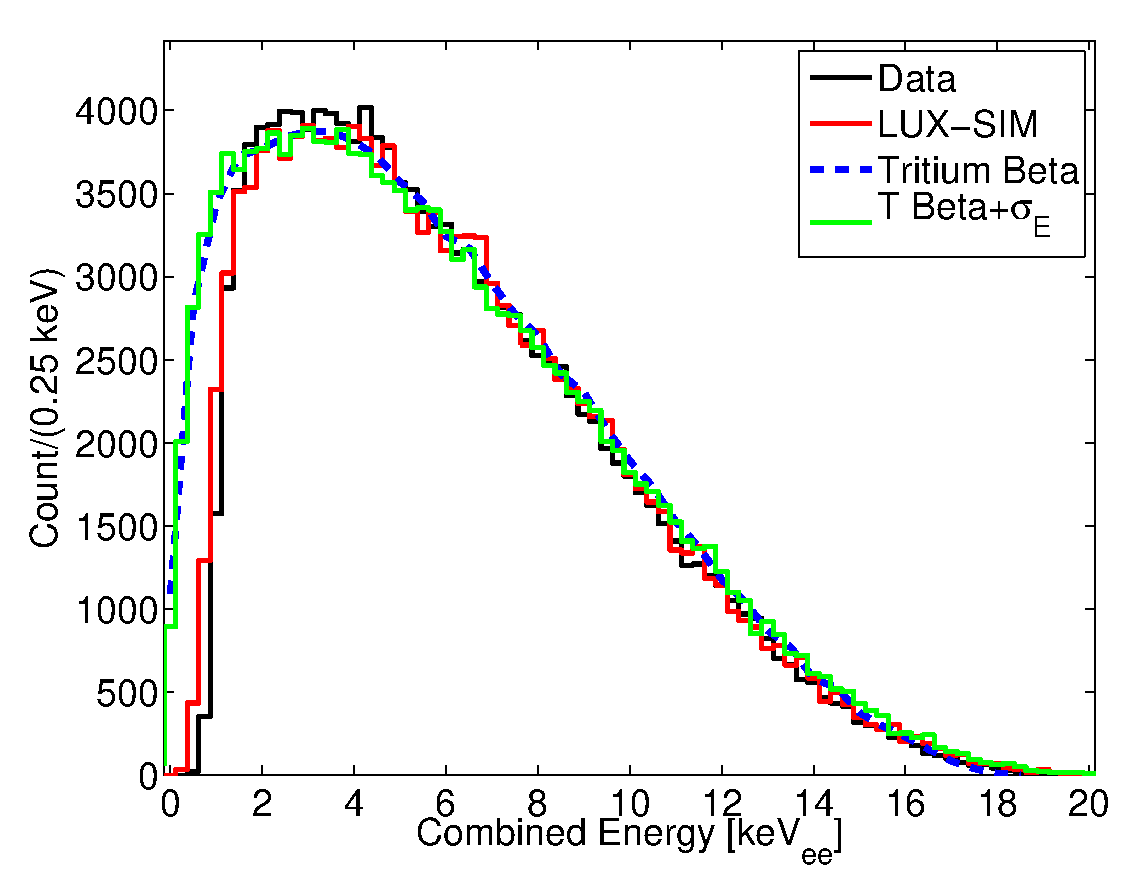
\includegraphics[width=70mm]{Chapter_Flucs/Figures/E_Spec/E_spec_compare_SIM.eps}
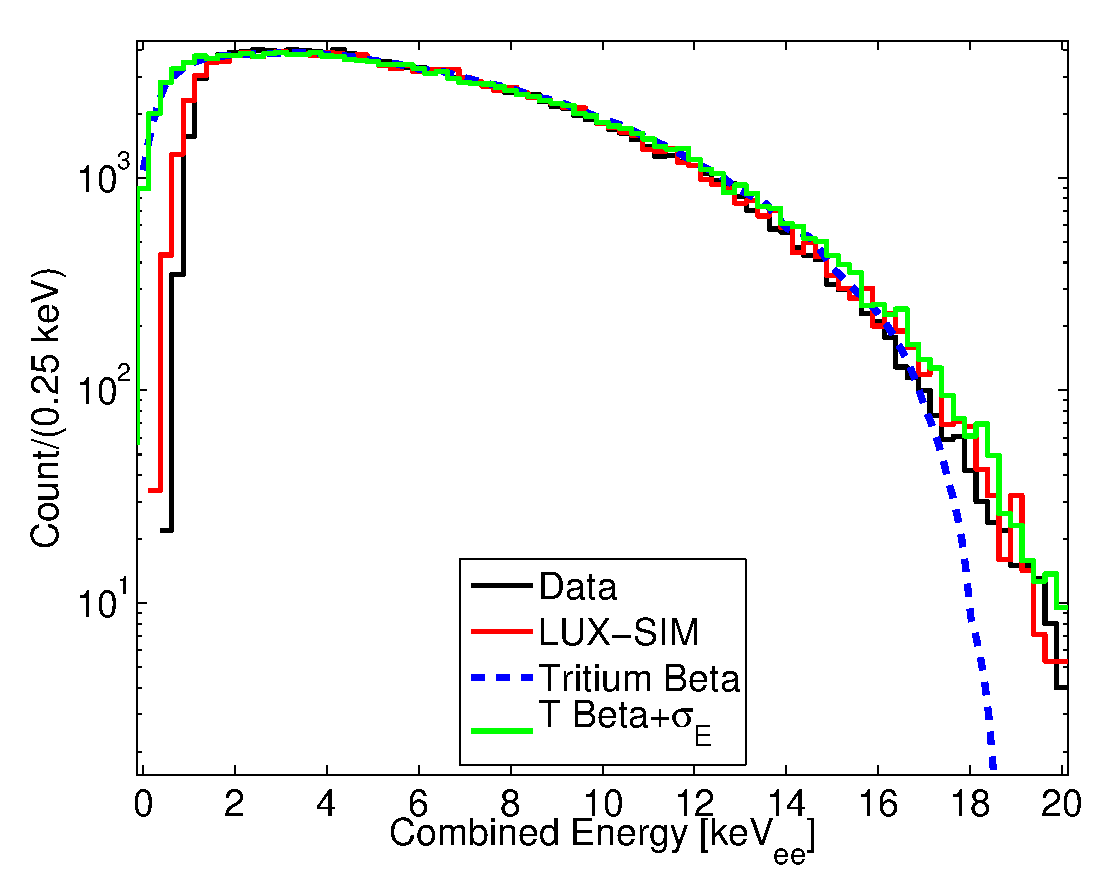
\includegraphics[width=70mm]{Chapter_Flucs/Figures/E_Spec/E_spec_compare_SIM_log_.eps}
\caption{The tritium energy spectrum reconstructed from the data using both Pulse Area and Spike count for S1. Along with LUX SIM, the true tritium beta spectrum and a tritium spectrum smeared with detector resolution. }
\label{fig:E_spec}
\end{figure}


 \begin{figure}[h!]\centering
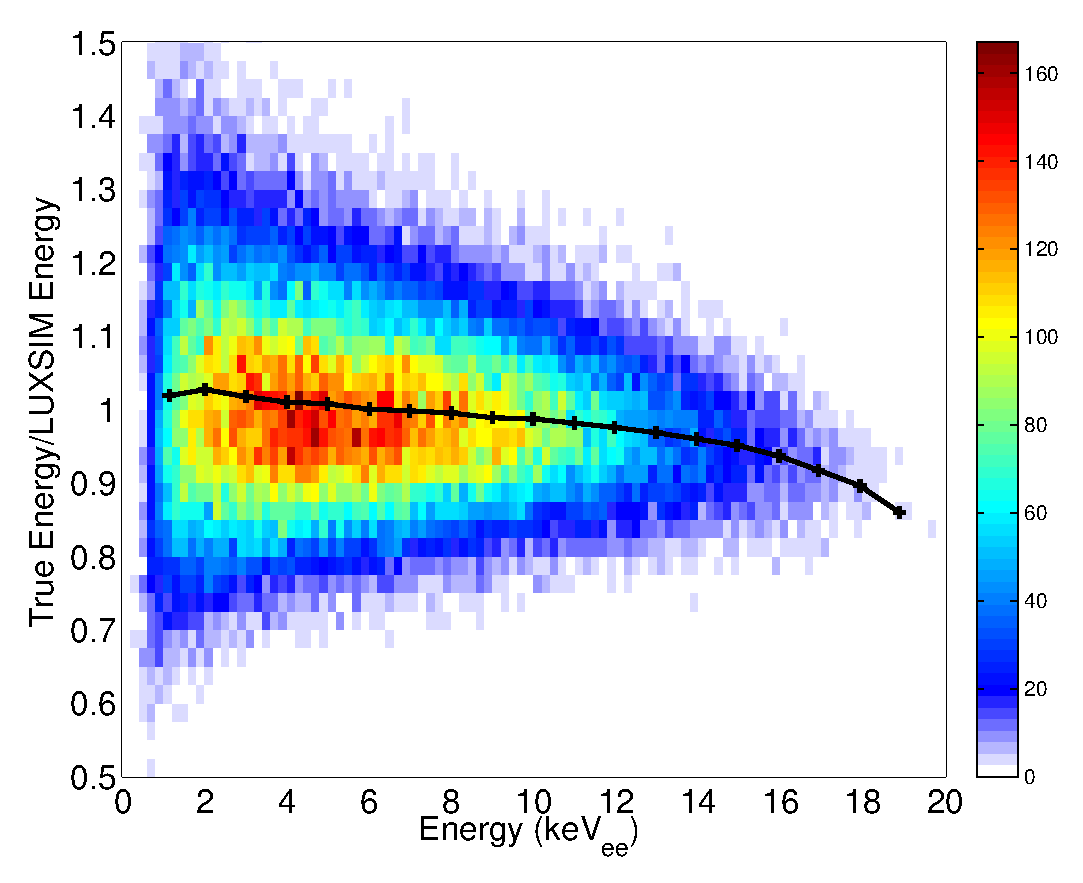
\includegraphics[width=70mm]{Chapter_Flucs/Figures/E_density_LUX_SIM_Tritium.eps}
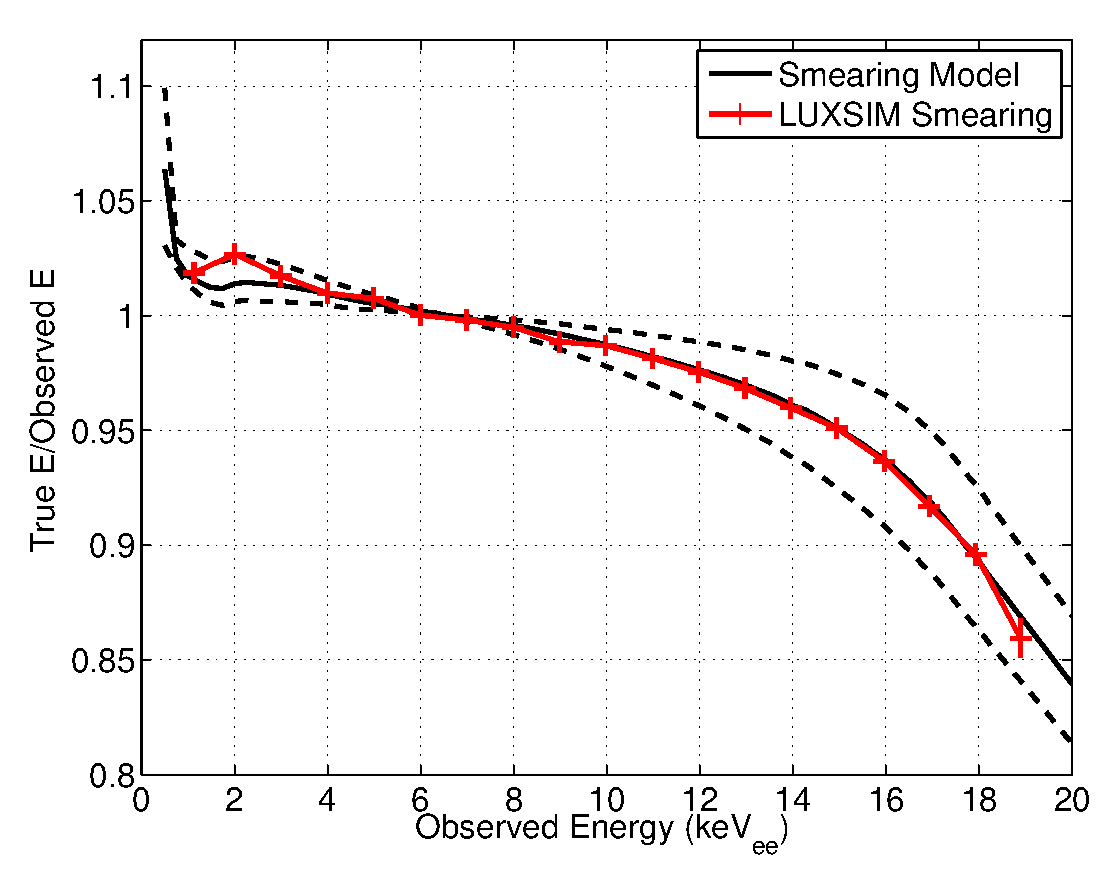
\includegraphics[width=70mm]{Chapter_Flucs/Figures/E_corr.eps}
\caption{Left, mapping from real Monte Carlo energy to observed energy after applying a finite resolution using LUXSIM. Right, comparing the correction determined from the Monte Carlo (Red) to the detector smearing model (black) given in equation \ref{eq:E_res}. The dashed lines represent the uncertainty in the measured value of F(E). The agreement is within errors from 1 to 18 keVee. The Energy threshold is near 1.0 $\rm keV_{ee}$.}
\label{fig:E_mapping}
\end{figure}

\subsection{LY, QY, $\rm \sigma R$ Result}

 The S1 and S2 spectral shape is not a good match with the light yield model from NEST, thus applying a correction to the observed means using NEST is not prudent. Fortunately, we see that both in the S1 and S2 region of interest were the majority of the tritium events occur the spectral shape correction is less than 10\%. Further, the reconstructed energy, uncorrected for spectral shape, is go to within 10\% as well. Knowing this we can move forward with extracting a more accurate light yield and recombination fluctuation accepting the small error in order to create a more accurate model than NEST to which then we can apply the spectral shape correction.

\newpage 

 \begin{figure}[h!]\centering
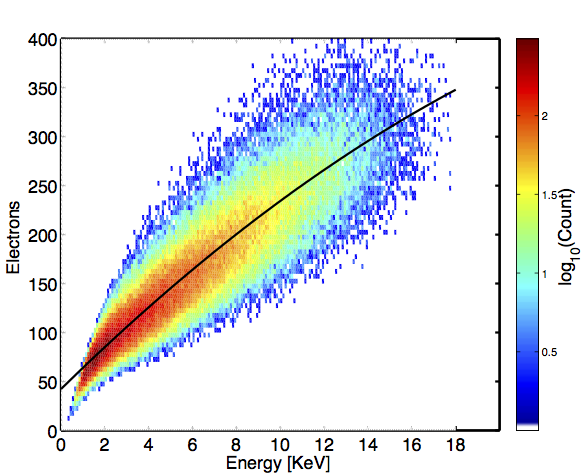
\includegraphics[width=70mm]{Chapter_Flucs/Figures/Iter0/n_electron_180_LY_QY_0.png}
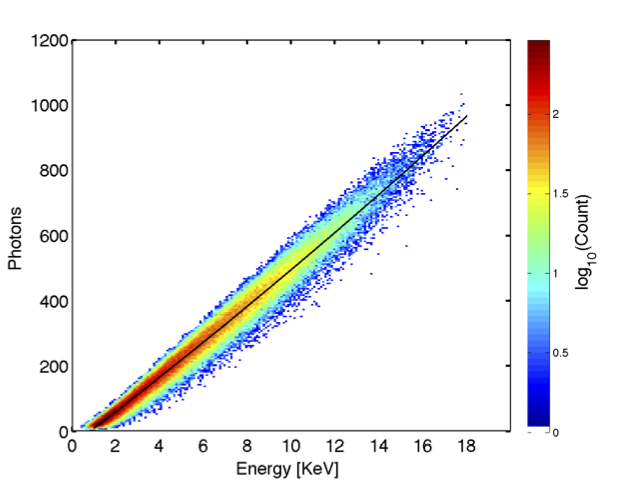
\includegraphics[width=70mm]{Chapter_Flucs/Figures/Iter0/n_photon_180_LY_QY_0.png}
\caption{Number of photons (left) and electrons (right) vs. energy from tritium data without spectral shape correction. The spread in quanta per energy bin is used to measure recombination fluctuations.}
\label{fig:LYQY_0}
\end{figure}

 \begin{figure}[h!]\centering
 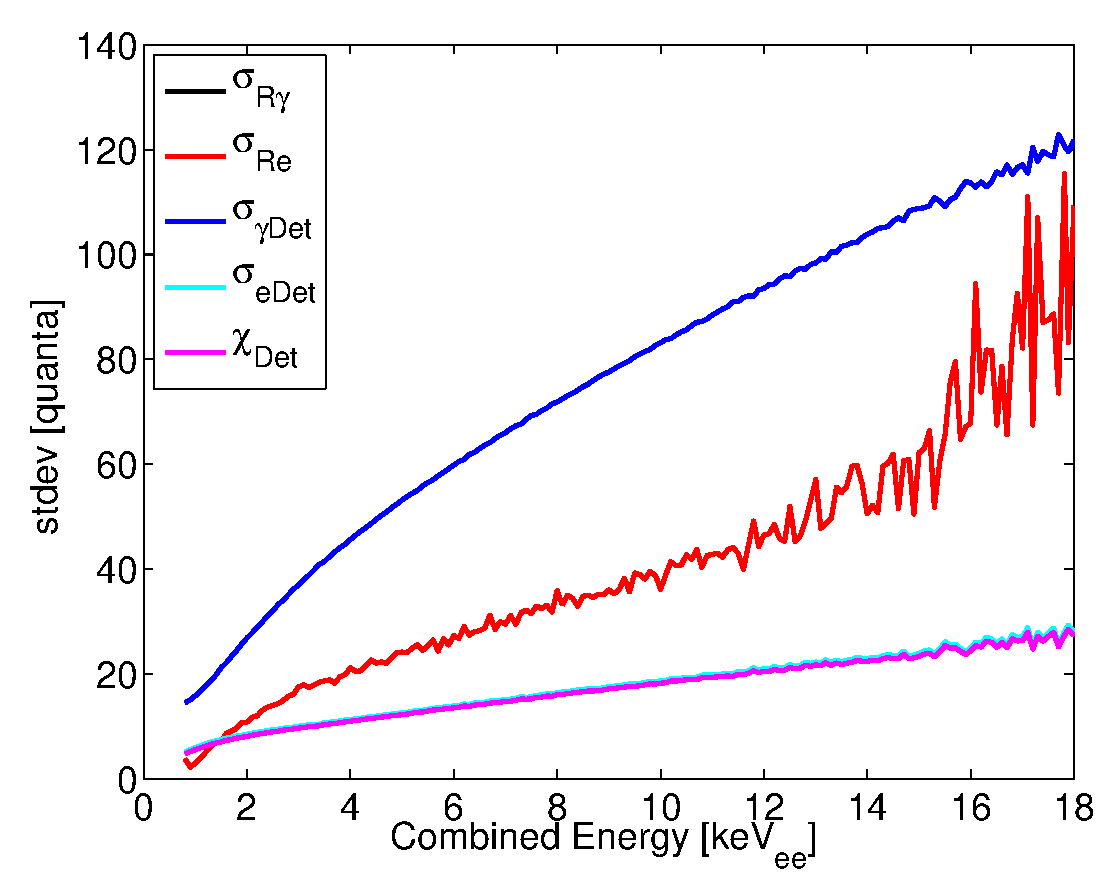
\includegraphics[width=90mm]{Chapter_Flucs/Figures/Iter0/std_fig_.eps}
 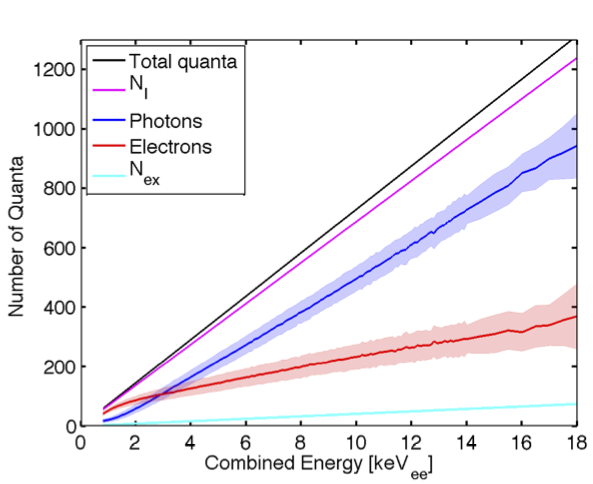
\includegraphics[width=72mm]{Chapter_Flucs/Figures/Iter0/quanta_LY_QY_0.png}
 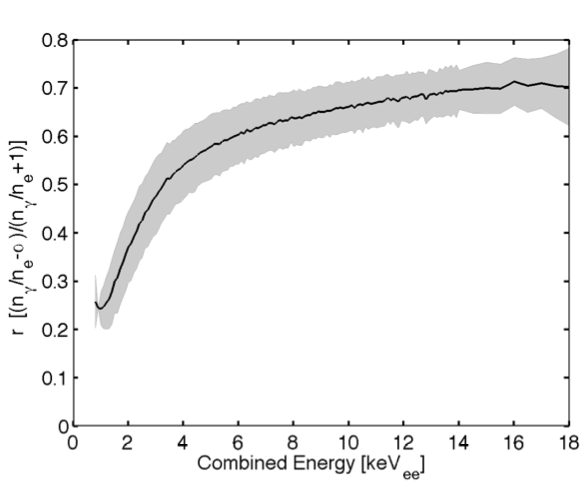
\includegraphics[width=72mm]{Chapter_Flucs/Figures/Iter0/R_LY_QY_0.png}
\caption{Top: Extracted recombination fluctuation from the tritium data from fluctuations in photons and electrons (Black and Red receptively). Bottom right: mean number of quanta in photons, electrons, ions, exitons vs. energy [keV] for the tritium calibrations. Bottom left: Recombination fraction and the one sigma (shaded) vs. energy [keV].}
\label{fig:Rec_0}
\end{figure}

Having extracted light yield (Photons/keV] and charge yield (electrons/keV) we compare the initial result from the tritium data to NEST, and is shown in figure \ref{fig:LYQY_0}. The disagreement between the data and the NEST yields was expected since previously the S1 and S2 tritium spectrum did not line up, in the previous section. Though the means do not match the measured light yield is within 1 sigma considering the large error in gains g1 and g2.

 \begin{figure}[h!]\centering
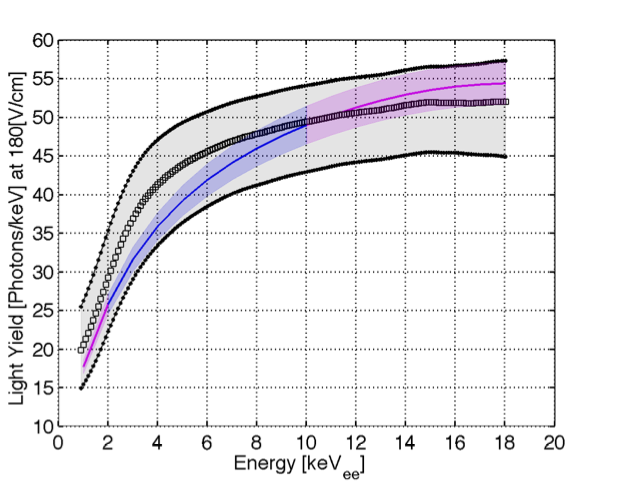
\includegraphics[width=82mm]{Chapter_Flucs/Figures/LYQY/LY_180_1sigBand_.png}
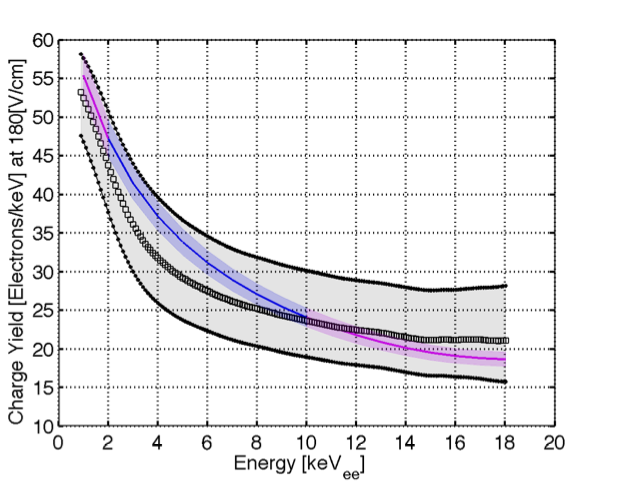
\includegraphics[width=82mm]{Chapter_Flucs/Figures/LYQY/QY_180_1sigBand_.png}
\caption{Light yield and charge yield from tritium data without spectral shape correction at 180 [V/cm] in black, the shaded region represents the one sigma uncertainty on g1 and g2. The NEST yield prediction and it's corresponding 1 sigma is shaded in blue. NEST interpolation in show in magenta to energies where the model is not vetted. }
\label{fig:LYQY_0}
\end{figure}


\newpage

\section{Measuring LY, QY, Recombination, Corrected for Spectral shape}

In the previous section we determined that the NEST model was not sufficient to produce a spectral shape correction for the tritium data. However, it was shown that and spectral shape correction is sufficiently small (less than 10\%) to extract light yield, charge yield and recombination from the tritium spectrum, using this information the model was improved and new simulations were produced. In this section we will take the information gathered in the previous section and apply the known detector resolution in order to create a spectral shape correction for the tritium S1 and S2. Having an improved model for NEST we can even determine the efficiency for  detecting tritium S1, S2 and the energy threshold, since the tritium spectrum still provides events well below the expected energy threshold of around 1.5 $\rm keV_{ee}$.


\subsection{Tritium S1 Correction}

Figure \ref{fig:S1_mapping_2} shows the application of smearing  from equation \ref{eq:S1_res} applied to the light yield extracted from the uncorrected tritium data with the data. The mapping for converting the observed S1 to the real S1 is shown in the figure. To calculate the correction we start with the extracted light yield, apply the measured g1, convolve it with a tritium beta spectrum and add in our first approximation of recombination fluctuations measured in equation \ref{eq:Inst_Fit}, given infinite detector resolution this is the spectrum the LUX detector would observe in S1 space. Knowing the dependance of detector resolution vs. the number of photons of a given event (equation \ref{eq:SigDet}) we can apply the model as outlined in \ref{sec:Smear} and calculate the shift from observed mean photons to real mean photons.

 \begin{figure}[h!]\centering
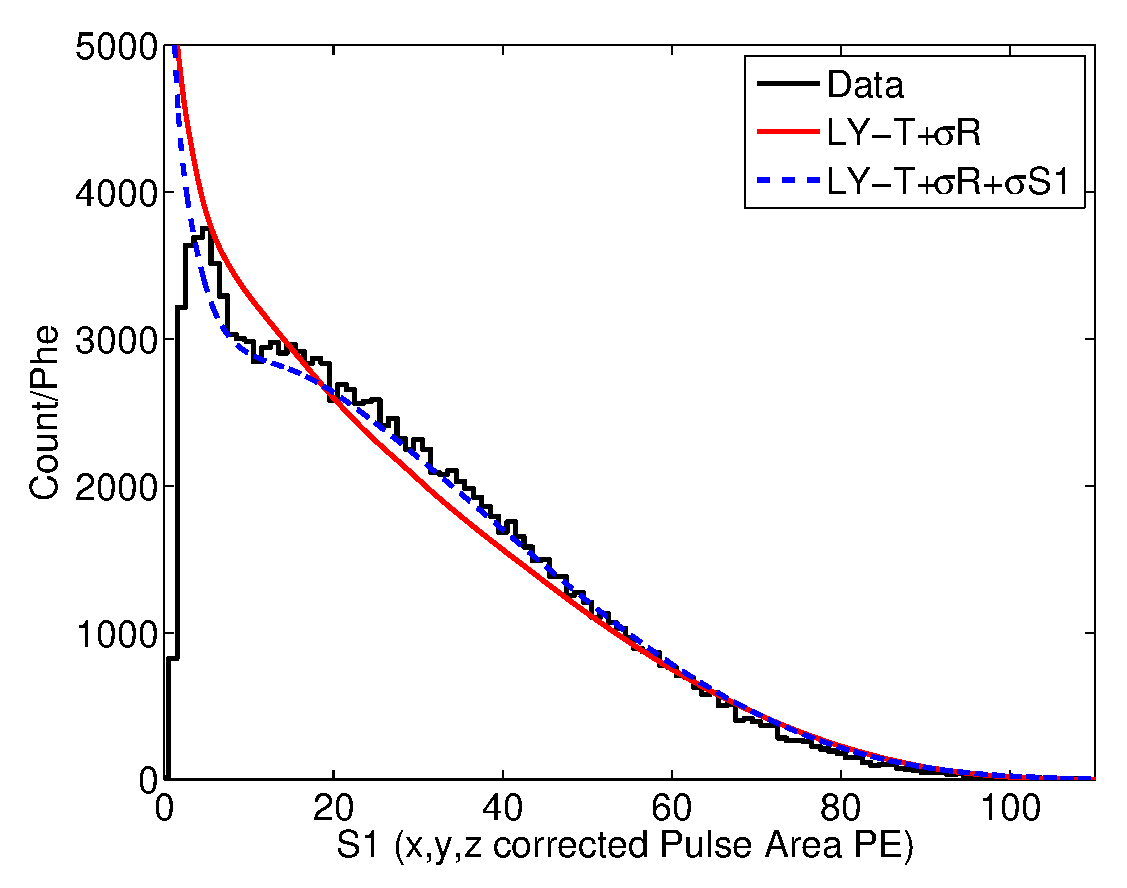
\includegraphics[width=70mm]{Chapter_Flucs/Figures/S1S2_Spectra/S1_spec_compare_iter1_.eps}
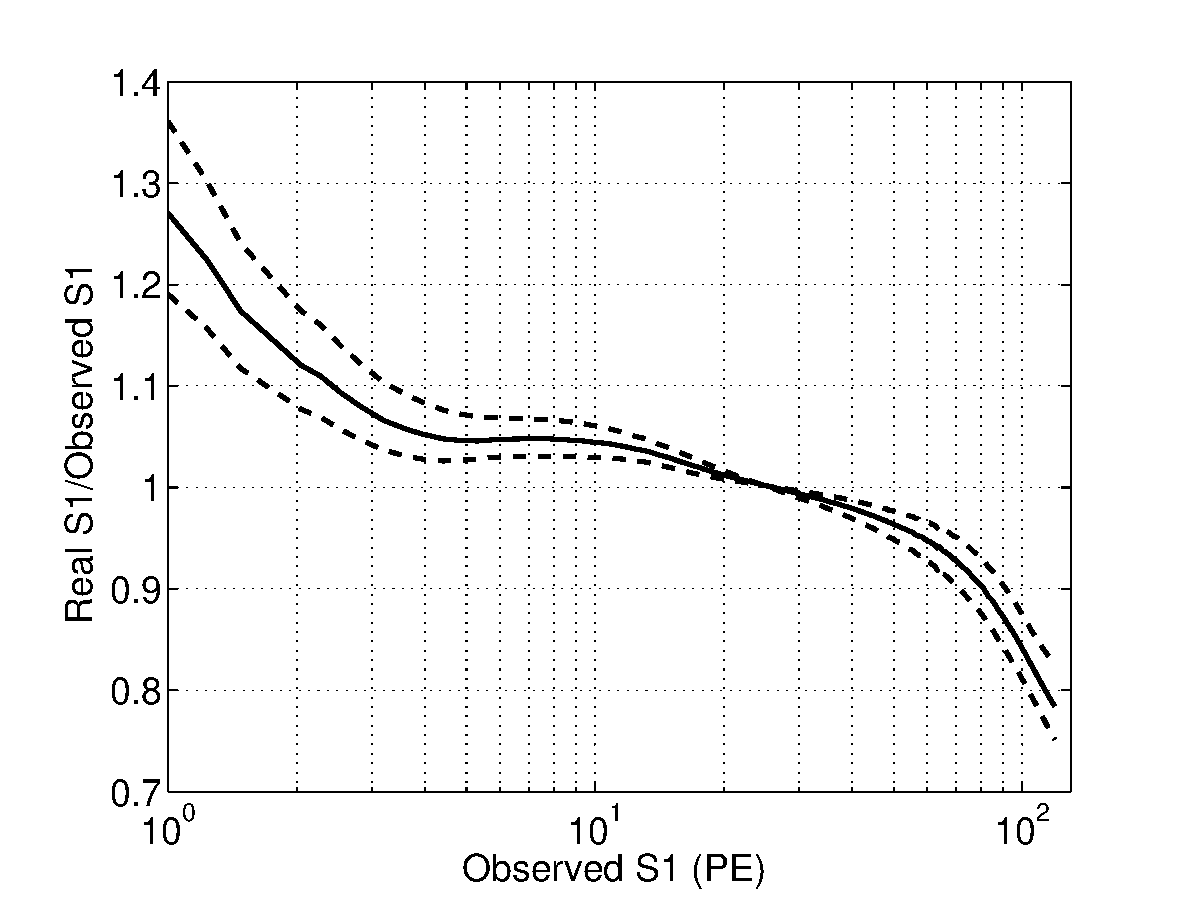
\includegraphics[width=70mm]{Chapter_Flucs/Figures/S1S2_Spectra/S1_corr_iter1_.eps}
\caption{Left: In Black, tritium data. In red, the spectrum after applying measured recombination fluctuations. In dashed blue is after applying recombination and finite detector resolution of equation. Left: Mapping of the observed mean, with finite resolution, to the mean with infinite resolution for a tritium photon spectrum. Bottom Right: The ratio of the real mean to the observed mean vs. the observed mean for a tritium photon spectrum. Note the S1 threshold at about 3 Phe in S1. }
\label{fig:S1_mapping_2}
\end{figure}

\subsection{Tritium S2 Correction}


Figure \ref{fig:S1_mapping_2} shows the application of smearing  from equation \ref{eq:S2_res} applied to the charge yield extracted from the uncorrected tritium data with the data. The mapping for converting the observed S2 to the real S2 is shown in the figure. To calculate the correction we start with the extracted light yield, apply the measured g2, convolve it with a tritium beta spectrum and add in our first approximation of recombination fluctuations measured in equation \ref{eq:Inst_Fit}, given infinite detector resolution this is the spectrum the LUX detector would observe in S1 space. Knowing the dependance of detector resolution vs. the number of electrons of a given event (equation \ref{eq:SigDet}) we can apply the model as outlined in \ref{sec:Smear} and calculate the shift from observed mean photons to real mean photons.

 \begin{figure}[h!]\centering
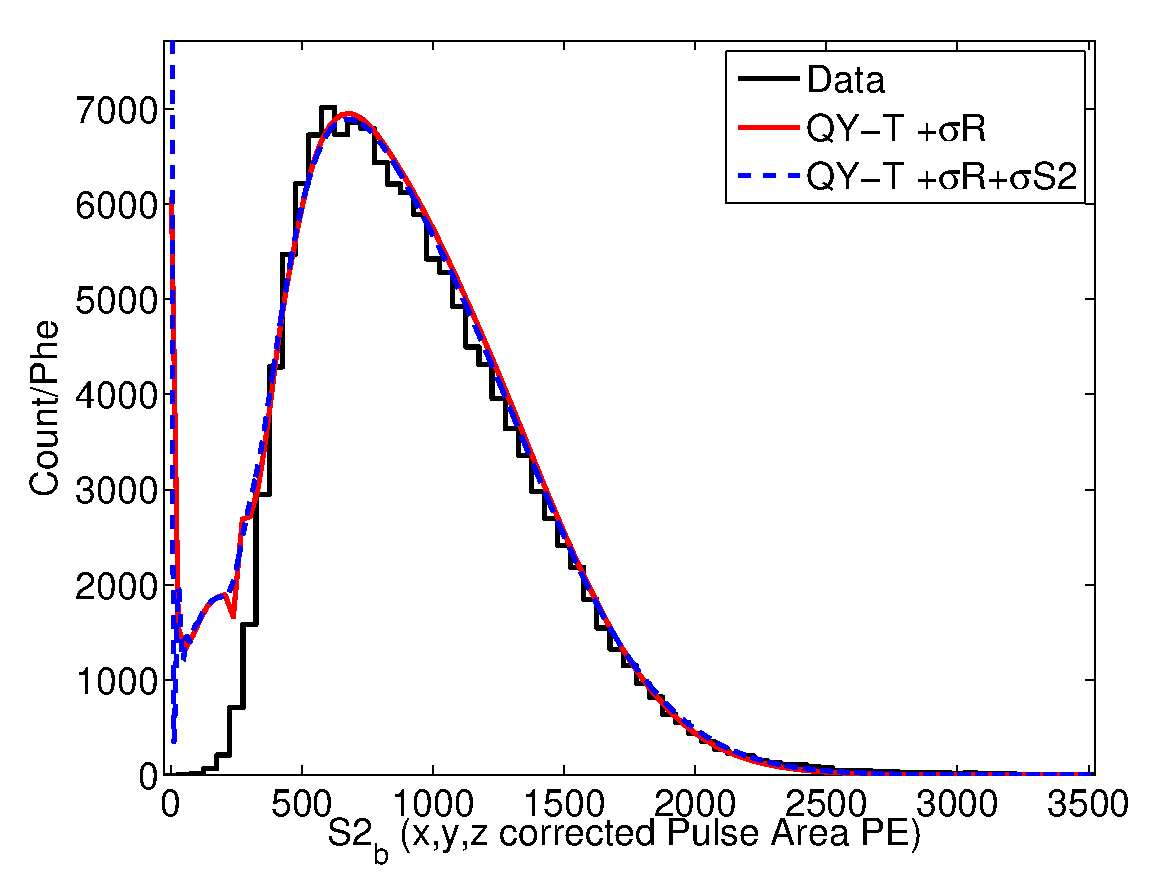
\includegraphics[width=70mm]{Chapter_Flucs/Figures/S1S2_Spectra/S2_spec_iter1_.eps}
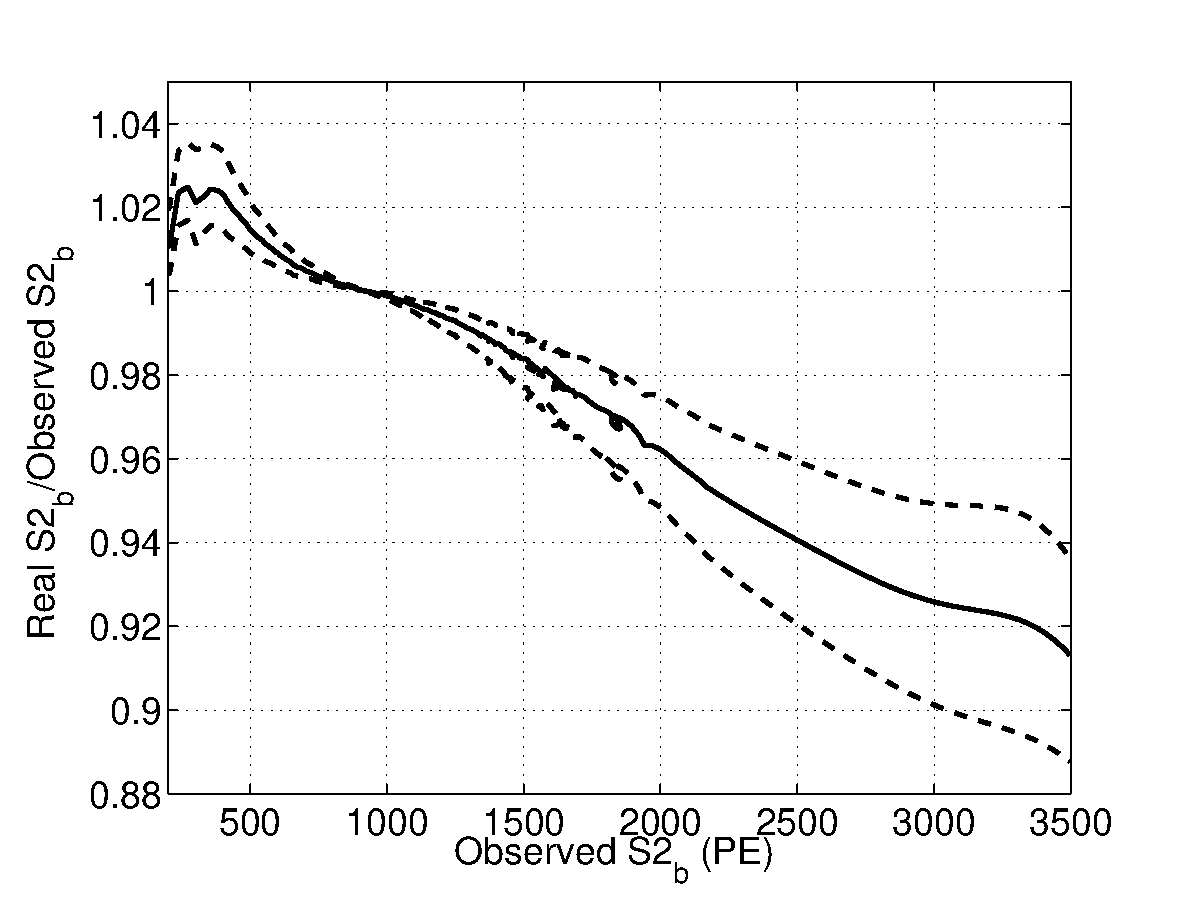
\includegraphics[width=70mm]{Chapter_Flucs/Figures/S1S2_Spectra/S2_corr_iter1_.eps}
\caption{Left: In Black, tritium data. In red, the spectrum after applying measured recombination fluctuations. In dashed blue is after applying recombination and finite detector resolution of equation. Left: Mapping of the observed mean, with finite resolution, to the mean with infinite resolution for a tritium photon spectrum. Bottom Right: The ratio of the real mean to the observed mean vs. the observed mean for a tritium photon spectrum. Note the S2 threshold at about 400  Phe. }
\label{fig:S2_mapping_2}
\end{figure}

\newpage

\section{Thresholds}

\begin{figure}[h!]\centering
 
\subcaptionbox{S1 \label{fig:3a}}{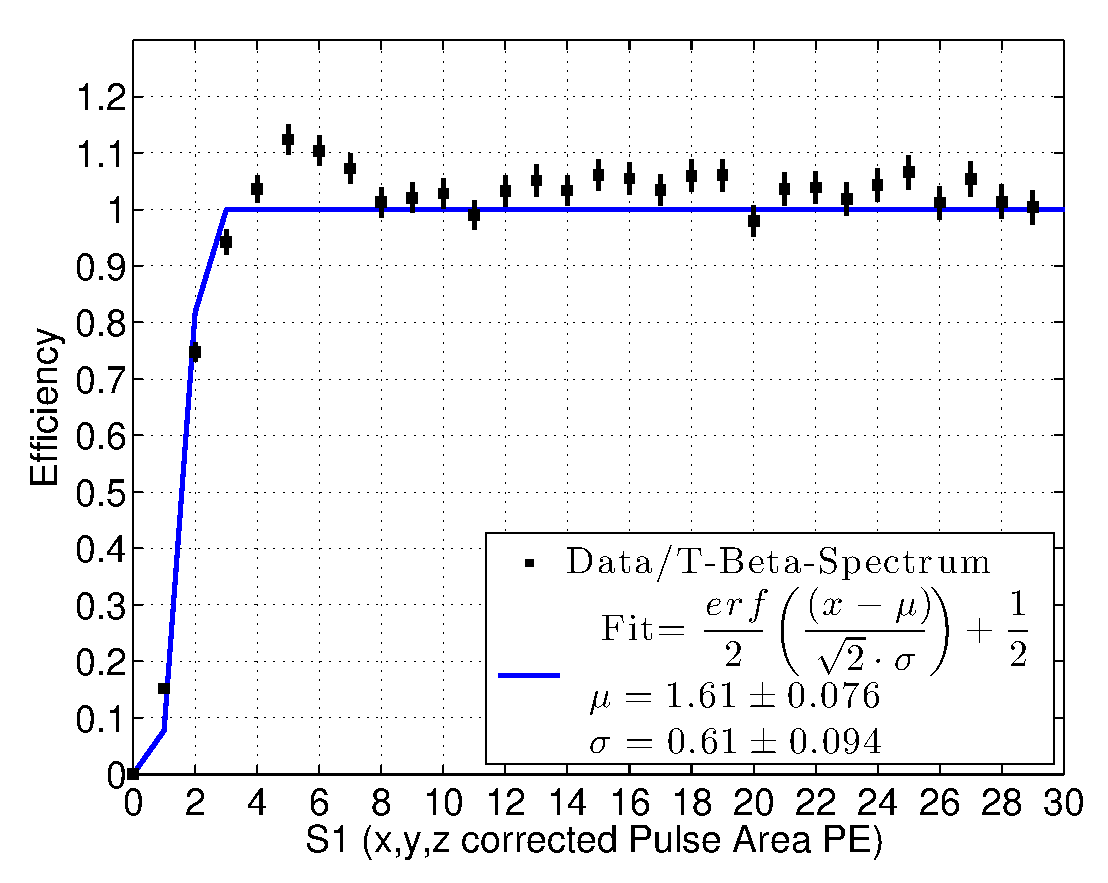
\includegraphics[width=70mm]{Chapter_Flucs/Figures/S1S2_Spectra/S1_Thres_.eps}}
\hfill
\subcaptionbox{$\rm S2_b$ (golden) \label{fig:3b}}{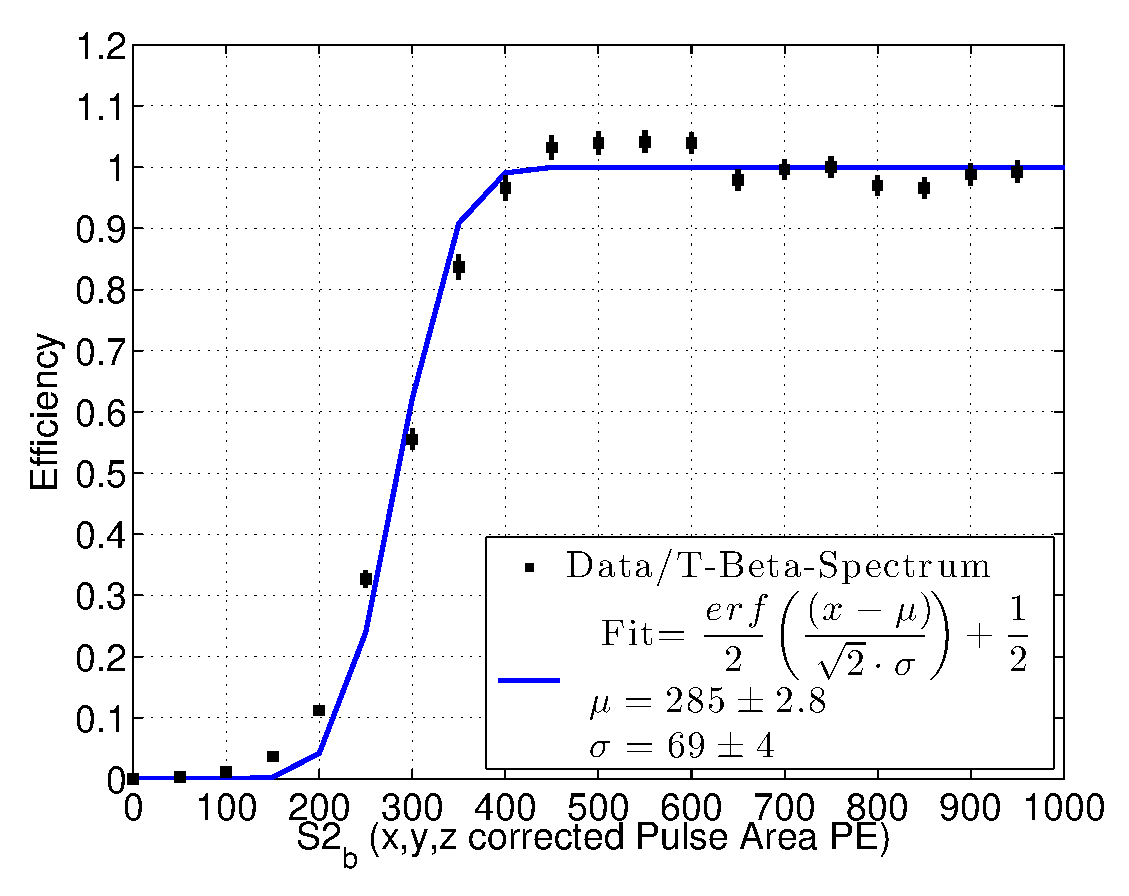
\includegraphics[width=70mm]{Chapter_Flucs/Figures/S1S2_Spectra/S2_Thres_.eps}}

\bigskip

\subcaptionbox{Combined Energy \label{fig:3c}}{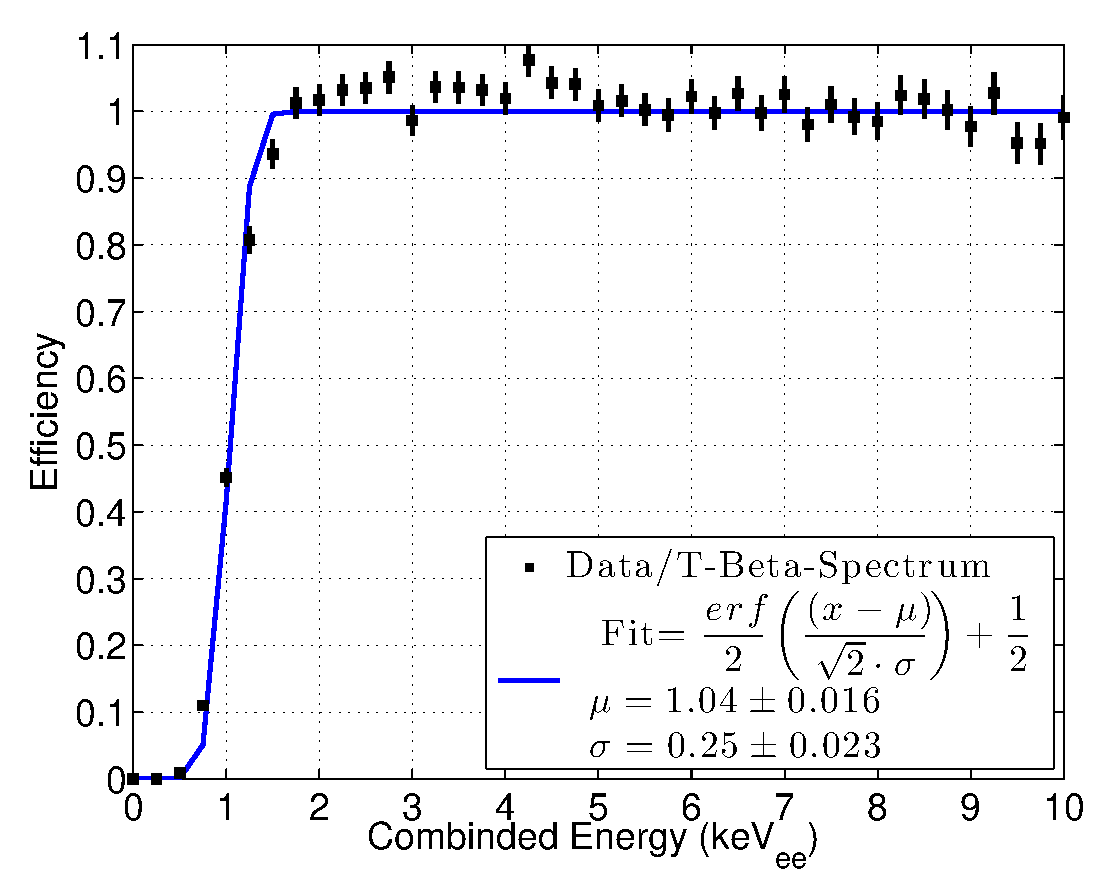
\includegraphics[width=70mm]{Chapter_Flucs/Figures/E_Spec/E_Thres_LY_QY_iter1.eps}}

\caption{Threshold calculated from difference of simulated Tritium S1, S2 and energy spectra. a) S1 b) $\rm S2_b$, c) E .}
\label{fig:Thres}
\end{figure}


\newpage

\section{Ionization and Scintillation Yield After Correction}

 
\newpage
 \begin{figure}[h!]\centering
 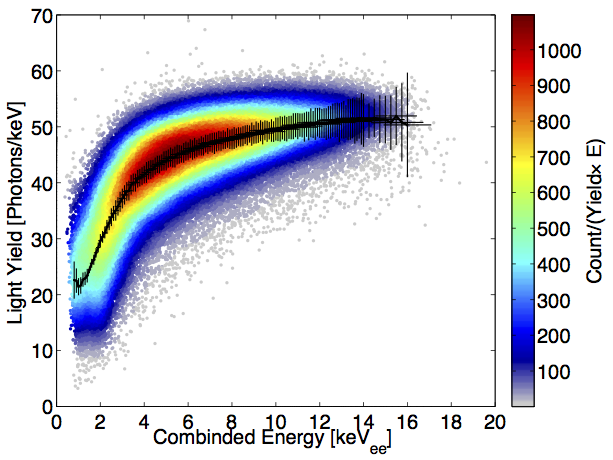
\includegraphics[width=82mm]{Chapter_Flucs/Figures/Iter1/LY_c_180_means_LY_QY_iter1.png}
 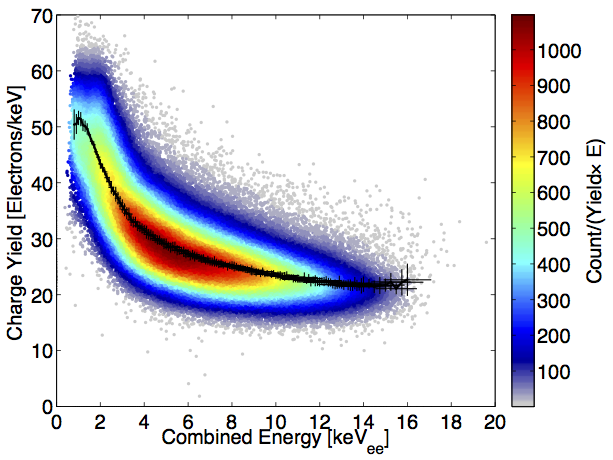
\includegraphics[width=82mm]{Chapter_Flucs/Figures/Iter1/QY_fid_means_LY_QY_iter1.png}
\caption{Extracting LY and QY from data corrected for spectral shape.}
\label{fig:LYQY_data}
\end{figure}


 \begin{figure}[h!]\centering
 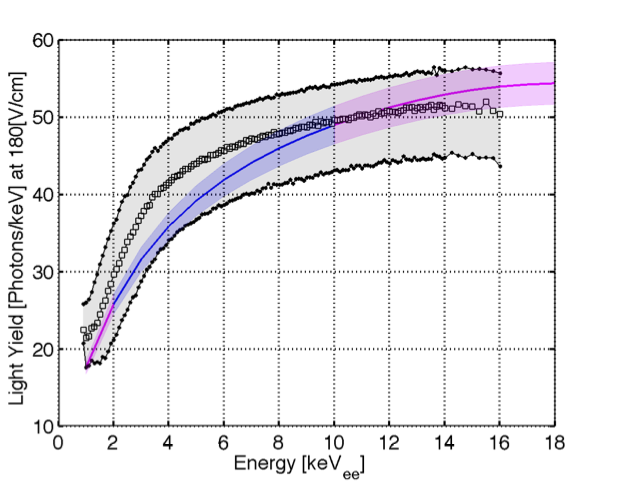
\includegraphics[width=82mm]{Chapter_Flucs/Figures/Iter1/LY_180__1sigBand_LY_QY_iter1.png}
 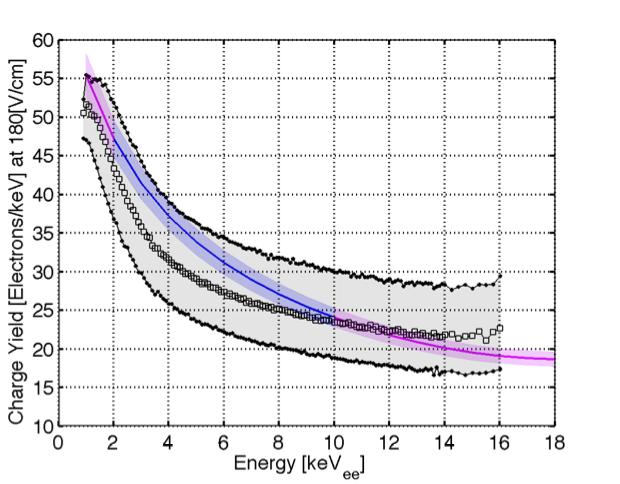
\includegraphics[width=82mm]{Chapter_Flucs/Figures/Iter1/QY_180_1sigBand_.png}
\caption{LY and QY from tritium data corrected for spectral shape along with the 1 sigma band of g1/g2. The blue and magenta curve are NEST extrapolation and interpolation, respectively.}
\label{fig:LYQY_data}
\end{figure}


\newpage

\section{The Standard Candle. Light Yield from $\rm^{83m}Kr$}

Quenching of scintillation yield vs. field has been  typically defined relative to 32.1 keV decay of $\rm^{83m}Kr$ at zero field \cite{Aprile_LY},\cite{Baudis}. $\rm^{83m}Kr$ first emits a 32.1 [keV] gamma followed by a 9.4 [keV] with a half life of 154 [ns] between the two (refs). The combined signal (41.6 [keV]) is found by the pulse finder in the majority of cases, using the standard WIMP search pulse gap setting of 500 ns. However, the combined signal is not useful as a standard calibration since the light yield from the second 9.4 keV decay depends strongly on decay time separation. The second 9.4 keV decay is effected by the presence of exitons from the initial 32.1 [keV] decay. See figure [ show LUX result]

Fortunately, the first 32.1 keV appears to have no time dependance as it decays in `relaxed' xenon without the presence of additional exitons \cite{Aprile_LY}. For purposes of light yield normalization at zero field the 32.1 keV gamma serves as a good low energy standard candle for xenon detectors.

There were two data sets in late 2013 that contain $\rm^{83m}Kr$ decays at zero field. Since the S2 (charge) signal is unavailable the top-bottom asymmetry, $\frac{top-bottom}{top+bottom} $, is used to define the Z coordinate for position dependent corrections. The XY correction is subdominant to the Z dependent correction for light yield. Figure [] shows the linear mapping from top-bottom asymmetry to detector depth (Z). With the Z correction applied the average pulse area (Phe) normalized to the detector center (241.6 mm below the gate grid) is found to be $\rm 267.4 \pm^{stat} 1.5 \pm^{sys} 5$. See Figure \ref{fig:ZeroField_Kr}.

 
 \begin{figure}[h!]\centering
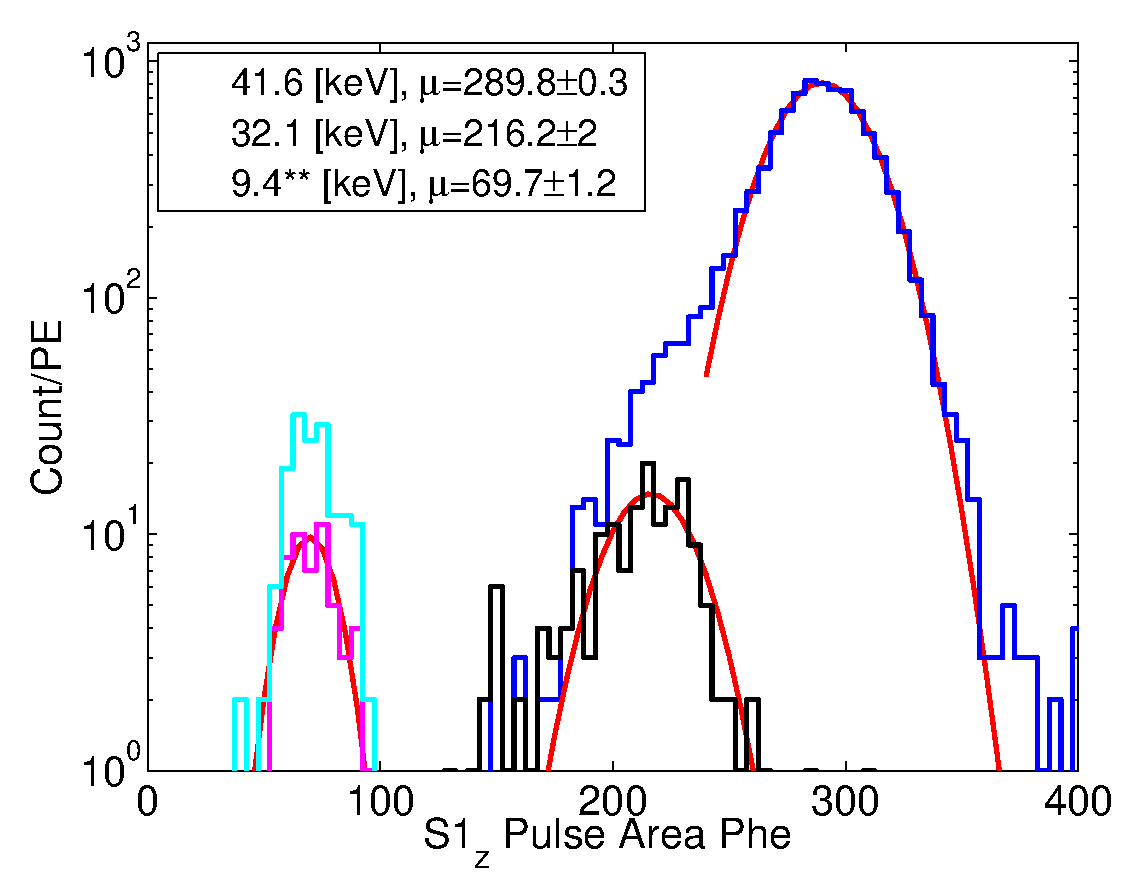
\includegraphics[width=72mm]{Chapter_Flucs/Figures/S1_Z_no_field_lux10_20131009T1358_cp09670} %old cp 6914
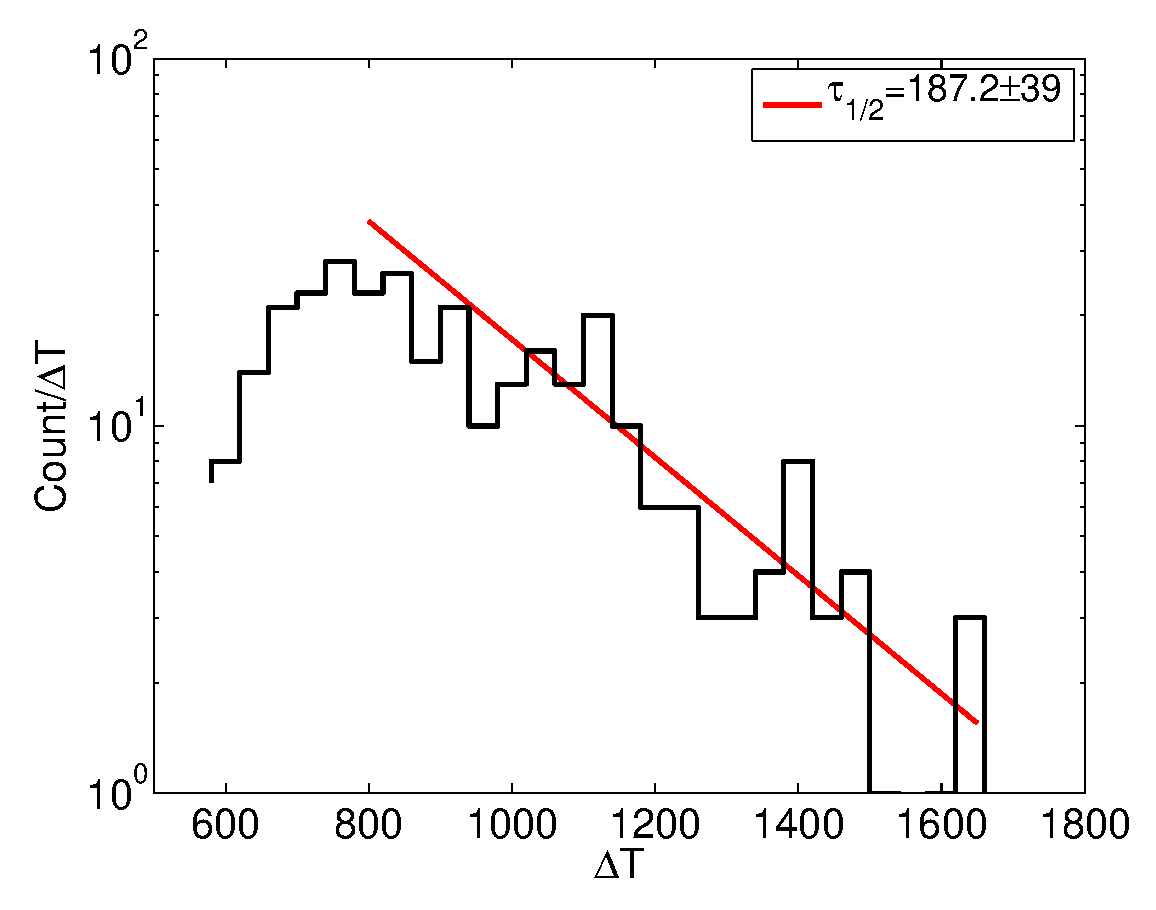
\includegraphics[width=72mm]{Chapter_Flucs/Figures/dT_no_field_2lux10_20131009T1358_cp09670}
\caption{Left: $\rm^{83m}Kr$ peaks at zero field. ** The 9.4 keV peak is fit only for events with a decay time separation greater than 1000 [ns]. Right: shows the timing separation between the 32.1 and 9.4 [keV] decays plotted above.}
\label{fig:ZeroField_Kr}
\end{figure}
 
\subsection{Field dependence of light yield from the 32.1 keV gamma of $\rm ^{83m}Kr$ }

Charge separation increases with drift field leading to less recombination for light production, causing scintillation yield to be quenched. See table \ref{table:kr32} for a list of the measured scintillation of the 32.1 keV gamma from $\rm ^{83m}Kr$, also includes the NEST predictions.

\renewcommand{\baselinestretch}{1}
\small\normalsize
\begin{table}[h!]
\begin{center}
\begin{tabular}{|c|c|c|c|c|c|}
\hline
Field	&S1			& Photons						& Yield 								&NEST	 \\
V/cm	& PE					& $\left<n_{\gamma}\right>$		& $\left<n_{\gamma}\right>$/keV	& $\left<n_{\gamma}\right>$/keV \\ \hline
0 		&	216.2 $\pm$ 5.0 	&2228.9 $\pm$ 50.5 &	69.4 $\pm$	1.6 	&	64.2 $\pm$ 3.2  \\ \hline
50 		&	195.0 $\pm$ 0.7 	&2010.3 $\pm$ 7.2   & 	62.6 $\pm$	0.2	&	59.8 $\pm$ 3.0 \\ \hline
100 	&	178.4 $\pm$ 0.7 	&1839.2 $\pm$ 	7.2	 &	57.3 $\pm$ 0.2 	&	55.8 $\pm$ 2.8 \\ \hline
170 	&  171.4 $\pm$ 0.9		&1767.0 $\pm$ 	9.2  &	55.0 $\pm$ 0.3 	&	51.9 $\pm$ 2.6 \\ \hline
\end{tabular}
\caption{Field dependance of the light yield form the 32.1 keV decay of $\rm^{83m}Kr$. The fields are calculated using a two dimensional model and not accounting potential charge accumulation on inner teflon panels.}
\label{table:kr32}
\end{center}
\end{table}
\renewcommand{\baselinestretch}{2}
\small\normalsize



%\begin{table}[h!]
%\begin{center}
%\begin{tabular}{|c|c|c|c|c|c|c|}
%\hline
%Field 	&41.6 [keV] 	& 32.1 [keV] 	& 9.4* [keV] 	&9.4** [keV] & S2	&S2 ** \\ 
% \[[V/cm]	&	S1[Phe]	&S1[Phe]	&S1[Phe]&		S1[Phe]		&S2[Phe]		&S1[Phe]  \\ \hline
%0 	&		359.9 $\pm$ 5	 			&267.4 $\pm$ 6.5 		&78 $\pm$ 2	 	&	 92.5$\pm$	6 		&	--  			& --	\\ \hline
%51 &		332.6 $\pm$ 1.4 			&246.7 $\pm$ 1.2 		&76.4 $\pm$ 0.5 	& 	86 $\pm$ 1		 &	3651 $\pm$ 5	& 3708 $\pm$ 11 \\ \hline
%105 &		316.8 $\pm$ 1.4 			&233.6 $\pm$ 1.4 		&72.9$\pm$ 0.5		 &	83 $\pm$ 1 			&	4357 $\pm$ &4399 $\pm$ 16 \\ \hline
%182	 & 		291.3 $\pm$ 1.4 			&212.3 $\pm$ 1.3		&68.8 $\pm$ 0.5 	&	79 $\pm$ 1 		&	4986 $\pm$ 5 	 &5048$\pm$ 13 \\ \hline
%\end{tabular}
%\caption{Field dependance of the light yield form the 32.1, 9.4 and combined 41.6 [keV] decay of $\rm^{83m}Kr$. The fields are calculated using a two dimensional model and not accounting potential charge accumulation on inner teflon panels. ** *}
%\end{center}
%\label{table:krAll}
%\end{table}